% TODO: remove numpy
% TODO: winnow; move CSV to EC section; add xticks; make country_data.py friendlier
% LAB 9: Matplotlib
%
% CSE/IT 107: Introduction to Programming
% New Mexico Tech
%
\documentclass[11pt]{cselabheader}
\usepackage{float}

%%%%%%%%%%%%%%%%%% SET TITLES %%%%%%%%%%%%%%%%%%%%%%%%%
\fancyhead[R]{Lab 9: Matplotlib}
\title{Lab 9: Matplotlib}

\begin{document}

\maketitle
\pagenumbering{roman}
\hrule

\begin{quote}
``The greatest value of a picture is when it forces us to notice what we
never expected to see.''
\end{quote}
\begin{flushright}
---John Tukey
\end{flushright}

\begin{figure}[H]
  \centering
  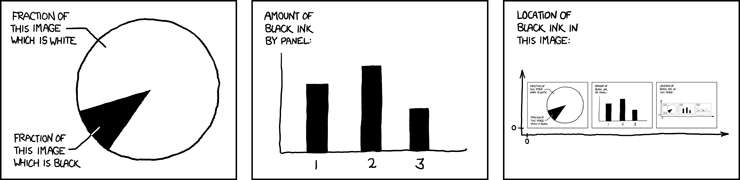
\includegraphics[width=\textwidth]{img/xkcd_self_description.png}
  \caption{Self description. \url{https://xkcd.com/688/}}
\end{figure}

\hrule

\pagebreak
\tableofcontents

\section*{Introduction}
\addcontentsline{toc}{section}{Introduction}
In this lab we will learn about generating 2D graphics using
Matplotlib.  This is a powerful Python library that can be used to
generate many kinds of visualizations such as scatter plots and
histograms. We will learn to about Python's list comprehensions and
how to create and manipulate Numpy arrays, which store numeric data.
There's also an overview of the CSV module, which makes it easy for
you to read and write CSV data files.  The key lesson of this lab is
learning to read Python library documentation. With this skill you can
learn to use many of Python's free and open-source libraries.

\pagebreak
\pagenumbering{arabic}
\section{Keyword Arguments}
Before we start, you should know about a commonly used Python feature
called keyword arguments. As you know, functions may take zero or more
required arguments, these are called \textsl{positional arguments}.
There is a special syntax that can be used to define \textsl{optional
arguments.}

For example, this function takes either one or two arguments. The second
argument has a default value of 5.

\begin{pyconcode}
>>> def f(fst, snd = 5):
...    return fst * snd
>>> f(10)
50
>>> f(10, 6)
60
>>> f()
Traceback (most recent call last):
  File ``<stdin>'', line 1, in <module>
TypeError: f() missing 1 required positional argument: 'fst'
\end{pyconcode}

An important feature is that keyword arguments may be labeled
and listed in any order when calling the function. For example,
the following function takes two keyword arguments. There are five
possible ways you can call this function.

\begin{pyconcode}
>>> def p(greeting="Hello", subject="world"):
...     return "{} {}".format(greeting, subject)
>>> p()
"Hello world"
>>> p(greeting="Goodbye")
"Goodbye world"
>>> p(subject="humans")
"Hello humans"
>>> p(greeting="Bonjour", subject="le monde")
"Bonjour le monde"
>>> p(subject="le monde", greeting="Bonjour")
"Bonjour le monde"
\end{pyconcode}

% \section{Numpy Arrays}
% Before we can use Matplotlib, we must learn about a new datatype:
% Numpy arrays.  These are efficient containers for numeric data and
% prefered when plotting data using Matplotlib. There are several ways
% to construct these arrays. The \pythoninline{numpy.array()} function
% can be used to convert a Python list into an array.
%
%   \begin{pyconcode}
% >>> import numpy
% >>> xs = numpy.array([1,2,3])
% array([1, 2, 3])
% >>> ys = numpy.array([8,4,7])
% array([8, 4, 7])
%   \end{pyconcode}
%
% The \pythoninline{numpy.linspace} can be used to create evenly spaced values.
% For example, if we want 10 points between 0 and 1 (inclusive), we can type:
%   \begin{pyconcode}
% >>> import numpy
% >>> numpy.linspace(0, 10, num=5)
% array([0, 2.5, 5, 7.5, 10])
%   \end{pyconcode}
%
% You can add or multiply two arrays element-by-element, and you can
% apply other mathematical functions to arrays. For example, the
% \pythoninline{numpy.sqrt} function can be used to find the square root
% of each element in the array.
%   \begin{pyconcode}
% >>> import numpy
% >>> xs = numpy.linspace(0, 1, num=5)
% array([0, 2.5, 5, 7.5, 10])
% >>> os = numpy.linspace(-20, 0, num=5)
% array([-20, -15, -10, -5, 0])
% >>> xs + os
% array([-20, -12.5, -5, 2.5, 10])
% >>> xs * os
% array([0, -37.5, -50, -37.5, 0])
% >>> numpy.sqrt(xs)
% array([0, 1.58113883, 2.23606798, 2.73861279, 3.16227766])
% >>> numpy.sin(os)
% array([-0.91294525, -0.65028784, 0.54402111, 0.95892427, 0])
%   \end{pyconcode}
%
% The \pythoninline{numpy.arange} function is similar to Python's
% \pythoninline{range} function. It improves on the built-function by
% generating values spaced by non-integers.
%
% \begin{pyconcode}
% >>> import numpy
% >>> numpy.arange(0, 10)
% array([0, 1, 2, 3, 4, 5, 6, 7, 8, 9])
% >>> numpy.arange(0, 12, 3)
% array([0, 3, 6, 9])
% >>> numpy.arange(0, 4, 0.5)
% array([0.0, 0.5, 1.0, 1.5, 2.0, 2.5, 3.0, 3.5])
% \end{pyconcode}

\section{List Comprehensions}
\subsection{Modifying Collections}
List comprehensions can be used to create lists where each element is the
result of some operations applied to each member of another sequence. For
example, if we want to make every string in a list of strings lowercase we can
use a for-loop:

\begin{pyconcode}
>>> strings = ["Python", "N.M."]
>>> result = []
>>> for string in strings:
...    result.append(string.lower())
... print(result)
["python", "n.m."]
\end{pyconcode}

List comprehensions are a more concise way of doing this:

\begin{pyconcode}
>>> result = [string.lower() for string in strings]
>>> print(result)
["python", "n.m."]
\end{pyconcode}

We can process more complicated elements with list comprehensions.
If we have a list of dictionaries containing lists, we can find the maximum
element in the list contained in each dictionary with this code:
\begin{pyconcode}
>>> data = [{'d': [1,2,3], 'label': "increasing"},
...         {'d': [0,0,1], 'label': "non-decreasing"}]
>>> [max(dictionary['d']) for dictionary in data]
[3, 1]
\end{pyconcode}

Dictionary comprehensions do exist and can be used to edit the keys and
values of a dictionary.

\subsection{Filtering Elements}
What if we want to exclude elements?
In this code, we take a list of words and keep all words of length greater
than 4:

\begin{pyconcode}
>>> strings = ['a', 'ab', 'abb', 'aab']
>>> result = []
>>> for string in strings:
...    if len(string) <= 2:
...        result.append(string)
... print(result)
['a', 'ab']
\end{pyconcode}

This code can be written more concisely by using an \pythoninline{if}
statement within a list comprehension.

\begin{pyconcode}
>>> strings = ['a', 'ab', 'abb', 'aab']
>>> [x for x in strings if len(x) <= 2]
['a', 'ab']
\end{pyconcode}

\subsection{Nested Comprehensions}
We can also write multiple \pythoninline{for} statements and
\pythoninline{if} statements in a list comprehension.
This example creates a list

\begin{pyconcode}
>>> result = [y / x for x in range(10) if x != 0 for y in range(10) if x != y]
\end{pyconcode}

These statements should be read from right to left. So the previous list
comprehension is the same as these nested for loops:

\begin{python3code}
result = []
for x in range(10):
    if x != 0:
        for y in range(10):
            if x != y:
                result.append(y / x)
\end{python3code}

\section{Matplotlib}
Matplotlib is a Python 2D plotting library which produces publication quality
figures in a variety of hardcopy formats and interactive environments.
There is a Matlab-like interface for generating most plots and an advanced
object oriented interface for generating many more graphics.

The \pythoninline{matplotlib.pyplot} library is commonly renamed
\pythoninline{plt} and the numpy library is aliased to
\pythoninline{np} for the sake of brevity.
\begin{pyconcode}
>>> import numpy as np
>>> import matplotlib.pyplot as plt
\end{pyconcode}

It's a good idea to keep the Matplotlib documentation on hand as you read these
examples. All of the following matplotlib functions are documented online at:
\begin{center}
\url{http://matplotlib.org/api/pyplot_api.html}
\end{center}

\subsection{Plotting Points with the \protect{\pythoninline{plot}} Function}

\pythoninline{plt.plot} is a versatile function that is used to plot
pairs of numeric values. The values on the x-axis are the first argument and
the y-axis values form the second argument. One of the lists must be in
increasing order.

\begin{pyconcode}
>>> import numpy as np
>>> import matplotlib.pyplot as plt
>>> plt.plot([1, 2, 3, 4], [10, -10, 40, 50])
>>> plt.show()
\end{pyconcode}

Note the \pythoninline{plt.show()} function shows everything drawn by
previously called plotting functions.  As of March, 2016 the
Matplotlib documentation for this function, colors, and line styles are
located at

\begin{center}
\url{http://matplotlib.org/api/pyplot_api.html#matplotlib.pyplot.plot}

\url{http://matplotlib.org/api/colors_api.html}

\url{http://matplotlib.org/api/lines_api.html#matplotlib.lines.Line2D.set_linestyle}
\end{center}

Matplotlib plots can be modified in many ways. The documentation has a
table of keyword arguments for this function. The columns are Property
and Description.  Let's try some of those. The \pythoninline{color},
\pythoninline{linestyle}, and \pythoninline{marker} keyword arguments
can be used to draw a differently styled line. See the documentation
for links to all possible colors, line styles and point markers.

\begin{pyconcode}
>>> import matplotlib.pyplot as plt
>>> plt.plot([1, 2, 3, 4], [10, -10, 40, 50],
...          color='red', linestyle='dashed', marker='o')
>>> plt.show()
\end{pyconcode}

\begin{figure}[H]
  \centering
  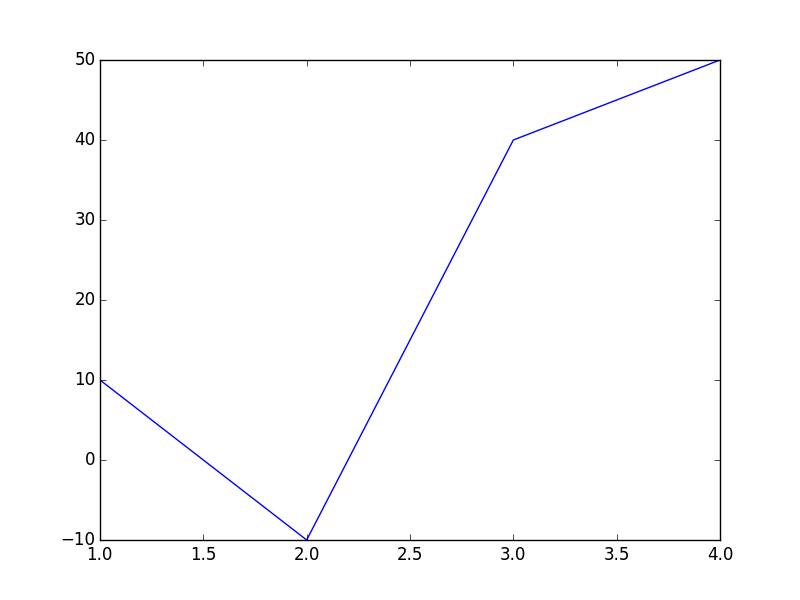
\includegraphics[width=0.49\textwidth]{img/matplotlib_plot1.png}
  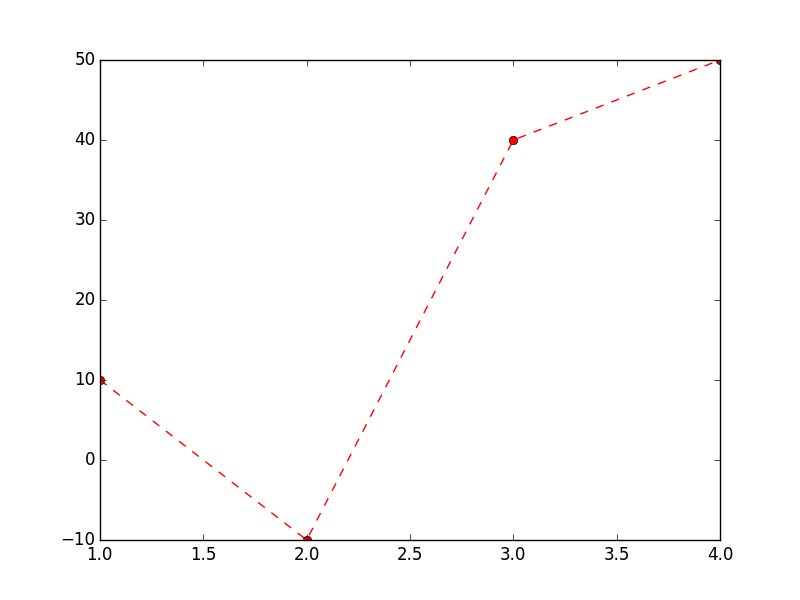
\includegraphics[width=0.49\textwidth]{img/matplotlib_plot2.png}
  \caption{Two separate plots of the same four points 1, 10; 2, -10;
3, 40; and 4, 50. In the right plot it is drawn with a red dashed line using
x's for markers.}
\end{figure}

\subsection{Histograms using the \protect{\pythoninline{hist}} Function}

Much of the features of the \pythoninline{matplilib.pyplot} functions are
enabled by passing keyword arguments. For example, the
%%% histogram

%%% copy docs
%%% READ DOCS

The histogram of an array, which shows how often a value occurs, can
be drawn using Matplotlib's \pythoninline{plt.hist()} function.  The
first argument is the array. Here is a demonstration of two possible
calls to draw the same data. The \pythoninline{bins} is used to draw
fewer bins of data. The histogram is rotated by setting
\pythoninline{orientation='horizontal'}.

\begin{pyconcode}
>>> import matplotlib.pyplot as plt
>>> plt.hist([1, 1, 1, 1.2, 1.3, 1.9, 1.9, 2, 2.1, 2.5])
>>> plt.show()
>>> plt.clf()
>>> plt.hist([1, 1, 1, 1.2, 1.3, 1.9, 1.9, 2, 2.1, 2.5]),
...          bins=4, orientation='horizontal', color='red')
\end{pyconcode}

The \pythoninline{plt.clf()} function is used to clear the current figure.
See the documentation for more keyword arguments to modify the histograms.

\begin{center}
\url{http://matplotlib.org/api/pyplot_api.html#matplotlib.pyplot.hist}
\end{center}

\begin{figure}[H]
  \centering
  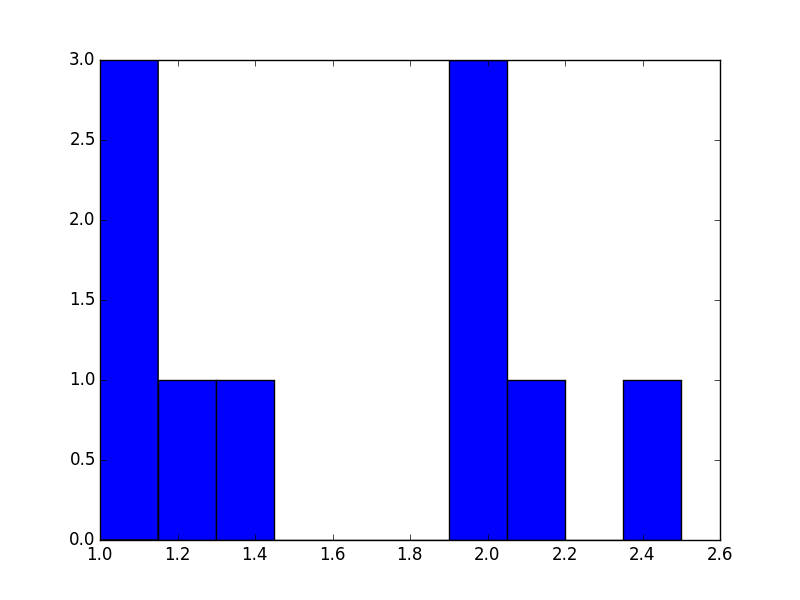
\includegraphics[width=0.49\textwidth]{img/matplotlib_hist1.png}
  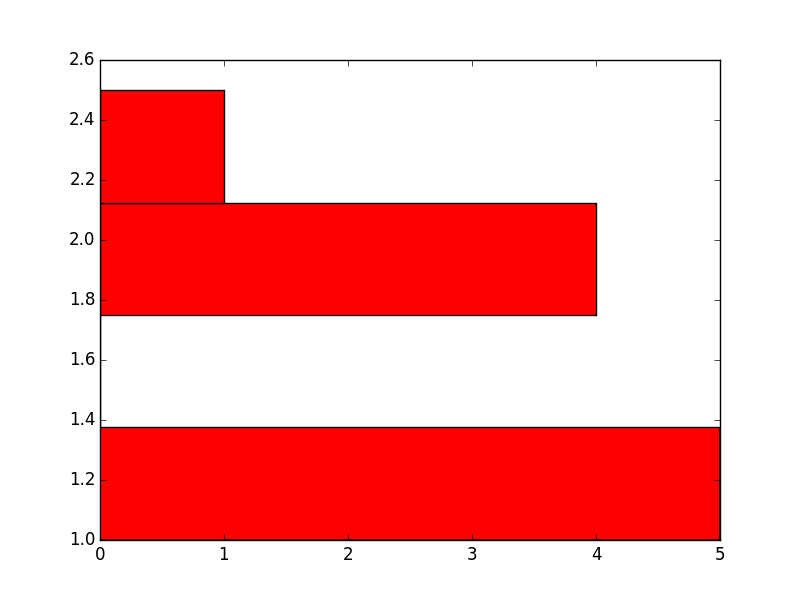
\includegraphics[width=0.49\textwidth]{img/matplotlib_hist2.png}
  \caption{Histograms of the same data. The right plot is rotated and has less
bins.}
\end{figure}

\subsection{Scatter plots with \protect{\pythoninline{scatter}} Function}
Scatter plots may be generated using the \pythoninline{plt.scatter} function.
These plots should be given three arguments \pythoninline{x, y, s}; these are
arrays indicating the x and y values of the data and the size of each data point.
The \pythoninline{c} and \pythoninline{alpha} keyword arguments can be used to
modify color and opacity of data points. Colors are automatically picked if an
array of values is given. Documentation available at

\begin{center}
\url{http://matplotlib.org/api/pyplot_api.html#matplotlib.pyplot.hist}
\end{center}

This plots data with ordered x-values between 0 and 10, randomly generated
y-values between 0 and 10, and sizes between 1200 and 10 with some variation.
The color scheme are automatically picked according to size.

\begin{pyconcode}
>>> import numpy as np
>>> import matplotlib.pyplot as plt
>>> x = np.linspace(0, 10, num=20)
>>> y = np.random.random(20) * 10
>>> sizes = np.linspace(1200, 30, num=20) + np.random.random() * 100
>>> plt.scatter(x, y, s=sizes, c=sizes, alpha=0.8)
>>> plt.show()
\end{pyconcode}

\begin{figure}[H]
  \centering
  
\includegraphics[width=0.8\textwidth]{img/matplotlib_scatter.png}
  \caption{A scatter plot with transparency and automatically selected color
scheme based on size.}
\end{figure}

\subsection{Bar Plots with the \protect{\pythoninline{bar}} Function}

Matplotlib can draw a plot of rectangles, each one bounded by the four edges:
\pythoninline{left}, \pythoninline{left + width}, \pythoninline{bottom}, and
\pythoninline{bottom + height}. Here's a demonstration using the
\pythoninline{color} and \pythoninline{edgecolor} keyword arguments.
Documentation is here:

\begin{center}
\url{http://matplotlib.org/api/pyplot_api.html#matplotlib.pyplot.bar}
\end{center}


The rectangles have randomly generated heights and the same width and space
between them.

\begin{pyconcode}
>>> import numpy as np
>>> import matplotlib.pyplot as plt
>>> lefts = np.arange(0, 100, 5)
>>> heights = np.random.random(20) * 50 + 10
>>> plt.bar(left=lefts, height=heights, width=4.5, bottom=0,
...         color='lightblue', edgecolor='blue')
>>> plt.show()
\end{pyconcode}

\begin{figure}[H]
  \centering
  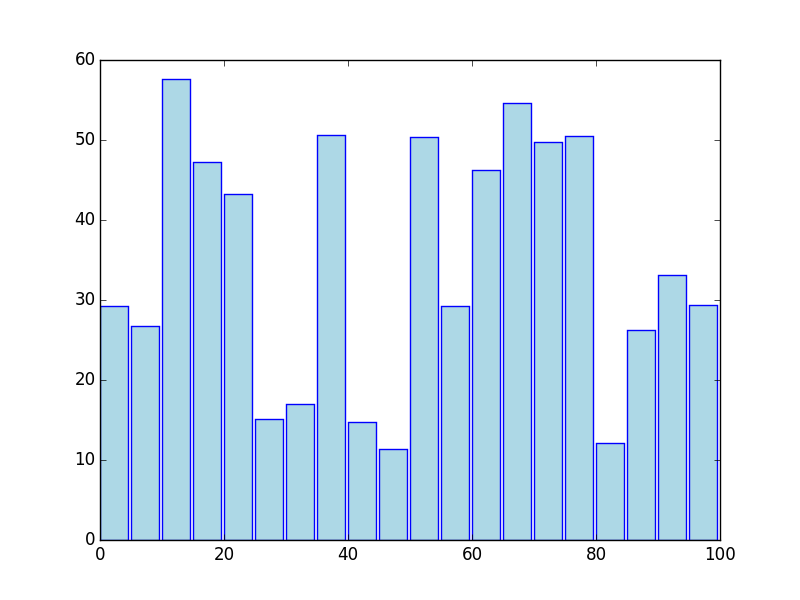
\includegraphics[width=0.7\textwidth]{img/matplotlib_bar.png}
  \caption{A bar plot where rectangles have the same width and separation.}
\end{figure}

\subsection{Drawing Many Plots with the \protect{\pythoninline{subplot}}
Function}

If you want to draw many plots in the same figure, use the
\pythoninline{plt.subplot} function to split the figure into several rows
and columns. The first and second arguments are the number of rows and columns.
The third argument is the figure number, this should be between 1 and
rows * columns. Documentation available at

\begin{center}
\url{http://matplotlib.org/api/pyplot_api.html#matplotlib.pyplot.subplot}
\end{center}

Here we draw 4 plots, three \pythoninline{plt.plot}s and one
\pythoninline{plt.hist} at the bottom corner.

\begin{python3code}
import numpy as np
import matplotlib.pyplot as plt
x = np.linspace(0, 10, num=20)
y = np.random.random(20)

plt.subplot(2, 2, 1)
plt.plot(x, y)

plt.subplot(2, 2, 2)
plt.plot(x, 0.5 * x ** 2)

plt.subplot(2, 2, 3)
plt.plot(x, y * x ** 2)

plt.subplot(2, 2, 4)
plt.hist(y)

plt.show()
\end{python3code}

\begin{figure}[H]
  \centering
  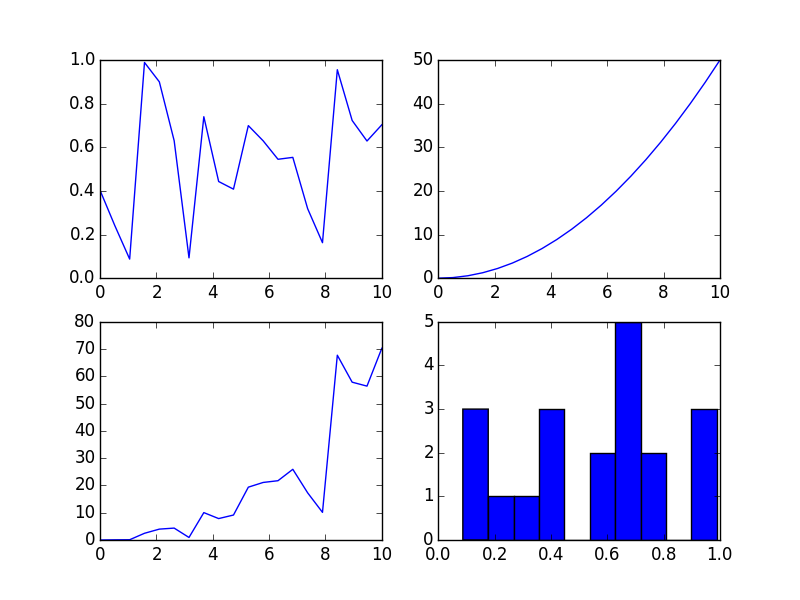
\includegraphics[width=\textwidth]{img/matplotlib_subplot.png}
  \caption{Four subplots.}
\end{figure}

\subsection{Describing your Plots}
See these links for documentation:
\begin{center}
\url{http://matplotlib.org/api/pyplot_api.html#matplotlib.pyplot.xlabel}

\url{http://matplotlib.org/api/pyplot_api.html#matplotlib.pyplot.ylabel}

\url{http://matplotlib.org/api/pyplot_api.html#matplotlib.pyplot.title}

\url{http://matplotlib.org/api/pyplot_api.html#matplotlib.pyplot.subplot}
\end{center}

Plots can be labeled and titled using the
\pythoninline{plt.xlabel},
\pythoninline{plt.ylabel},
and \pythoninline{plt.title} functions.
Here's an example:

\begin{python3code}
import numpy as np
import matplotlib.pyplot as plt
x = np.linspace(0, 50, num=20)
y = np.random.random(20) * x + x

plt.plot(x, y)
plt.xlabel('Time spent coding')
plt.ylabel('Winning')
plt.title('Data plot.')
plt.show()
\end{python3code}

What if you want to call attention to an individual data point? Then
you should consider the \pythoninline{plt.annotate} function to add
annotations to plots.  In this example we indicate the maximum y-value
in a randomly generated set of data: This code produces a labeled,
annotated plot.


Annotation text is set with \pythoninline{s}. The arrow is styled
using the \pythoninline{arrowprops} argument.  The \pythoninline{xy}
and \pythoninline{xytext} keyword arguments are used to place the
arrow and text.

\begin{python3code}
import numpy as np
import matplotlib.pyplot as plt
x = np.linspace(0, 50, num=20)
y = np.random.random(20) * x + x

# find maximum
maximum_index = np.argmax(y)
maximum = y[maximum_index]

plt.plot(x, y)
plt.xlabel('Time spent coding')
plt.ylabel('Winning')
plt.title('Data plot.')

# add annotation at maximum point
plt.annotate(s='Maximum value is {:.3}'.format(y[maximum_index]),
             xy=(x[maximum_index], y[maximum_index]),
             xytext=(x[maximum_index] * 0.6, y[maximum_index] * 0.9),
             arrowprops={'arrowstyle': "wedge,tail_width=0.25"})

plt.show()
\end{python3code}

\begin{figure}[H]
  \centering
  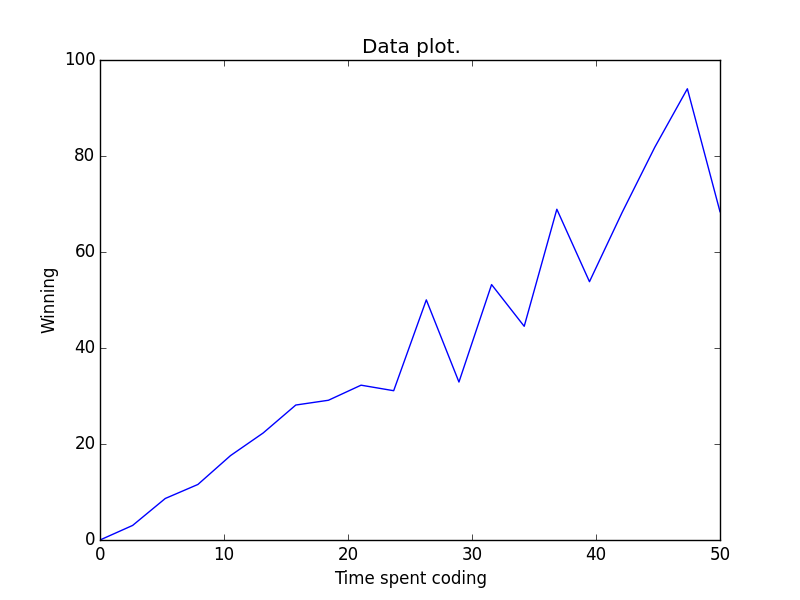
\includegraphics[width=0.49\textwidth]{img/matplotlib_labeled1.png}
  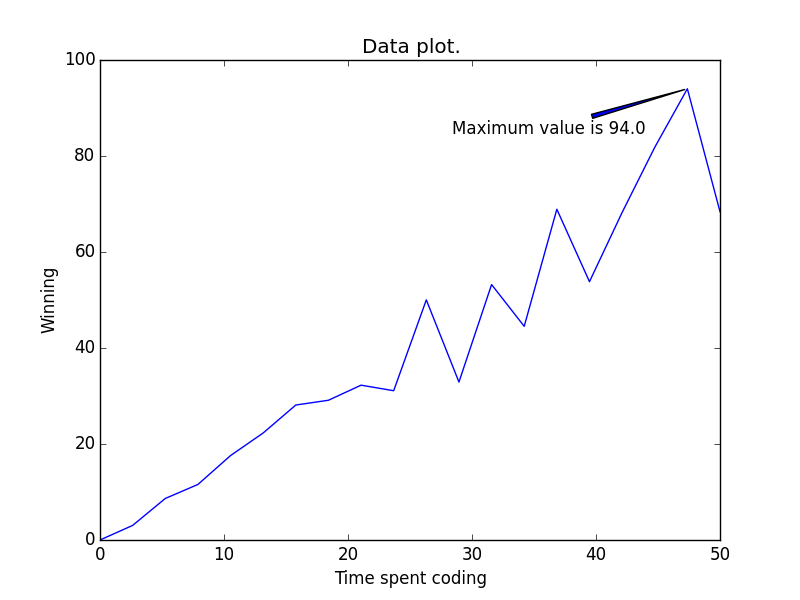
\includegraphics[width=0.49\textwidth]{img/matplotlib_labeled2.png}
  \caption{Labeled and titled plots. One of them using Matplotlib
annotations to show the median point...}
\end{figure}

\subsection{Subplots and Annotations}

Here's an example where subplots have annotations and titles.

\begin{python3code}
import numpy as np
import matplotlib.pyplot as plt
x = [1, 2, 3, 4, 5]
y1 = [4, 8, 2, 6, 0]
y2 = [14, 2, 8, 0, 1]

plt.subplot(1, 2, 1)
plt.plot(x, y1)
plt.annotate(s='Here is an 8', xy=(2, 8), xytext=(3,7),
             arrowprops={'arrowstyle': "wedge,tail_width=0.25"})
plt.title('Dataset 1')

plt.subplot(1, 2, 2)
plt.plot(x, y2)
plt.annotate(s='Here is another 8', xy=(3, 8), xytext=(2,9),
             arrowprops={'arrowstyle': "wedge,tail_width=0.25"})
plt.title('Dataset 2')

plt.show()
\end{python3code}

\begin{figure}[H]
  \centering
  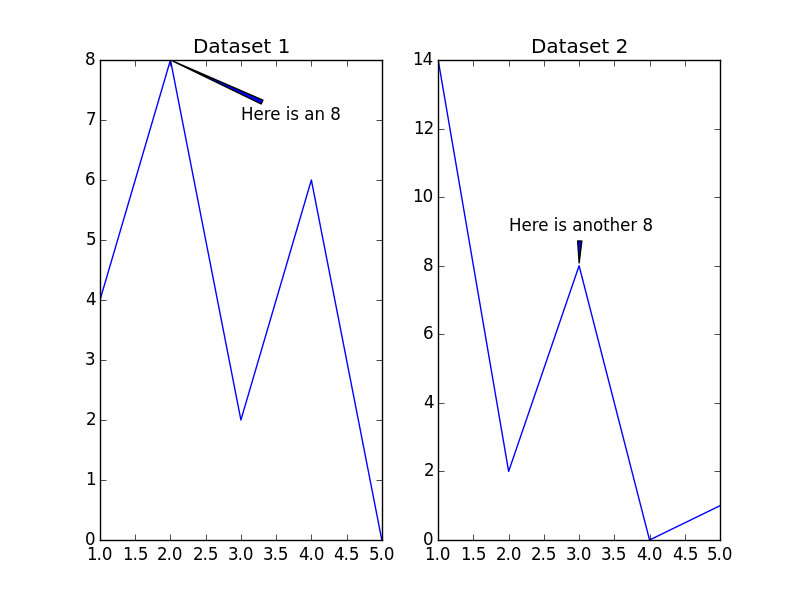
\includegraphics[width=\textwidth]{img/matplotlib_labeledsubplot.png}
  \caption{Annotated subplots.}
\end{figure}

\subsection{Overlaying Plots}
Plots may be overlayed by calling plot functions multiple times.
For example, here are plots of two data sets on the same figure.
There is also a line drawn at y=8.

\begin{python3code}
import numpy as np
import matplotlib.pyplot as plt
x = [1, 2, 3, 4, 5]
y1 = [4, 8, 2, 6, 0]
y2 = [14, 2, 8, 0, 1]

plt.plot(x, y1)
plt.plot(x, y2)
plt.plot([1,5], [8,8])
plt.title('Datasets 1 and 2')

plt.show()
\end{python3code}

\begin{figure}[H]
  \centering
  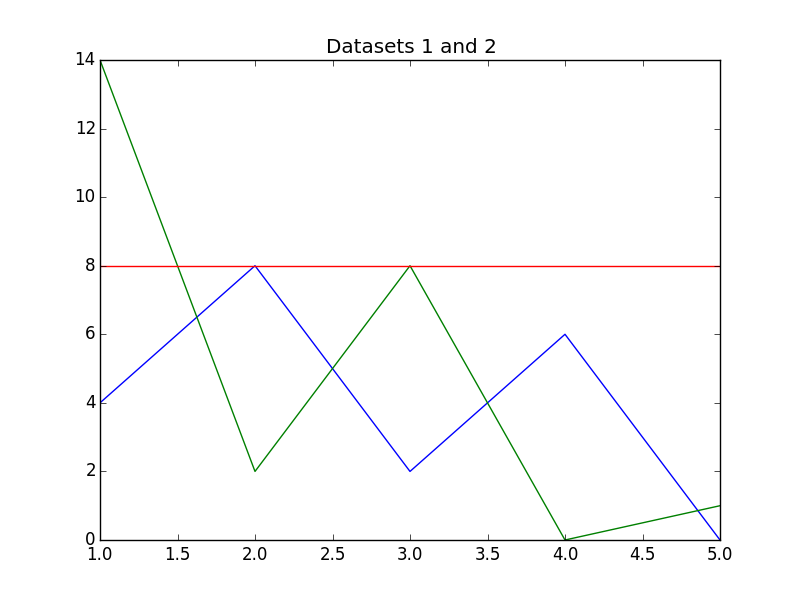
\includegraphics[width=\textwidth]{img/matplotlib_overlayed.png}
  \caption{Annotated subplots.}
\end{figure}

\section{Exploring APIs}
An important part of this lab is reading module documentation. You
have already seen two third party modules (Matplotlib and Numpy), and
built-in modules such as \pythoninline{math}. Almost every good Python
module has good documentation and if you want expertise in a module,
you should start reading its documentation.  For example, Matplotlib
supports animation, image rendering, stream plots, error plots,
contour plots, log scaled axis, and many other features. You can see
examples and detailed specifications in the Matplotlib docs.

\subsection{Other Libraries}
Other powerful, third-party and well-documented Python modules include
\begin{inparaenum}
\item \textsl{Scrapy:} a web crawling library.
\item \textsl{Newspaper:} an Easy to use natural language processor and news downloader.
\item \textsl{astropy:} astronomy and astrophysics packages.
\item \textsl{vtk:} highly functional 3D visualization library.
\item \textsl{pillow:} the friendly fork of the Python Imaging Library.
\item \textsl{OpenCV:} a computer vision library.
\item \textsl{Django:} used to deliver and manage dynamic websites; powers many large websites.
\end{inparaenum}

Visit their websites for information on usage and installation.
Here's a list of more interesting libraries:
\begin{center}
\url{https://github.com/vinta/awesome-python}
\end{center}

\newpage
\section{Exercises}
\begin{ex}[plotpoints.py]
Plot the following points. Add labels, a title, and an annotation to the plot
as shown in the example. Make sure to draw a dashed blue line.
The annotation contains the text ``max'' and is located at the point (2, 20).
The annotation text must be slightly below and the arrow connecting the text
and point must be black and have width set to 2.

\begin{python3code}
x = [1,2,3,4,5]
y = [10,20,15,5,-10]
\end{python3code}

\begin{center}
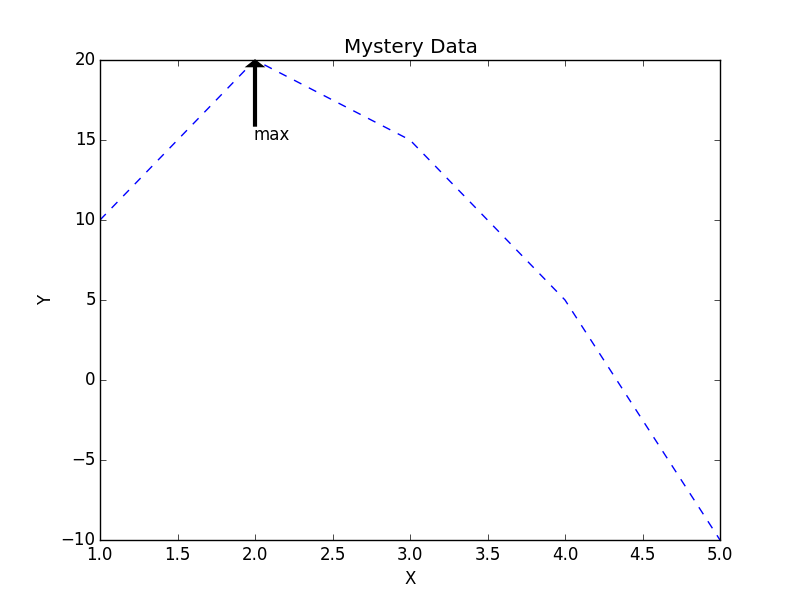
\includegraphics[width=0.5\textwidth]{img/basic.png}
\end{center}
\end{ex}

\begin{ex}[plotscores.py]
  This exercise relies on the \texttt{readscores.py} file from the File I/O
  lab. You may also rewrite that code using the CSV module.

  Write a program that generates the following charts:
  \begin{enumerate}
    \item A histogram of average ACT scores with bins of size $1$ between a
      score of $18$ and $24$.
    \item Two bar charts that compare the composite ACT score with the
      total score of all 3 SAT tests for all 51 states/territories.
      Normalize the data so that both bar charts have the same maximum points.
      Do this by dividing by the maximum possible SAT and ACT points.
      Each SAT section is out of 800 points, while the ACT is out of 36 points.
    \item Produce the same chart as in part 2, but only for states in which
      less than 50\% take the ACT and more than 50\% take the SAT. (There
      should be 21 states/territories like this.)
  \end{enumerate}

  A double bar graph may be created by calling the \pythoninline{plt.bar}
  plotting function multiple times with different data, you may also use
  \pythoninline{plt.subplot}s. Remember to label your axes and title your graph.
\end{ex}

\begin{infobox}{Supplementary Files}
The \texttt{actsat.txt} file is available on canvas as a lab 7 file.
\end{infobox}

\begin{ex}[plotcountries.py]
Use matplotlib to draw scatter plots relating worldwide life expectancy,
income per person, and population for the years 2010 and 1960.

You may access the data by completing the extra credit or by importing
\texttt{country\_data.py}. The data looks something like:

\begin{python3code}
data = {
 'Afghanistan': {1960: {'expectancy': 35.6846,
                        'gdp': 1206.0,
                        'population': 8994793.0},
                 2010: {'expectancy': 54.8,
                        'gdp': 1637.0,
                        'population': 27962207.0}},
 'Akrotiri and Dhekelia': {1960: {'expectancy': None, ...
\end{python3code}

Notice the special value \pythoninline{None} is present.
To check if a variable \pythoninline{x} is \pythoninline{None},
type \pythoninline{x == None} or \pythoninline{x is None}.
You are required to:

%%% TODO easier data format?
To convert a dictionary into a list, you may use the use the
\pythoninline{.items()} function. It returns a list of item and value tuples.

\begin{pyconcode}
>>> expectancy = [{'country': country, 'expectancy: cdata[1960]['expectancy']}
...                   for country, cdata in data]
[{'country': 'Afghanistan', 'expectancy': 35.6846}, ...
\end{pyconcode}

\begin{enumerate}
\item Draw a scatter plot with x and y coordinates set to income and life
expectancy. If there is a \pythoninline{None} value, replace it with the
minimum income or the minimum life expectancy.

\item The area of each data point should be related to the population of every
country. You can choose how to scale the data, but to make it look like the
example, you may use:
\begin{python3code}
scaled_pop = 800 * pop / max(pop)
\end{python3code}

\item The scatter plots must be labeled and titled. X label: ``Income'', y
label: ``Life expectancy'', title: ``Year (year of data)''.

\item Annotate China, Russia, United States, and Afghanistan as shown.
Annotations should have different coordinates and text coordinates.
You can get an arrow like in the example with this property:
\begin{python3code}
arrowprops={'arrowstyle': 'wedge,tail_width=0.25', 'color': 'black'}
\end{python3code}

\item Draw dashed red lines at the mean and at the max life expetancy.
The np.mean and Python's max functions are useful for this.
\end{enumerate}

Here is the plot for the 2010 data:
\begin{center}
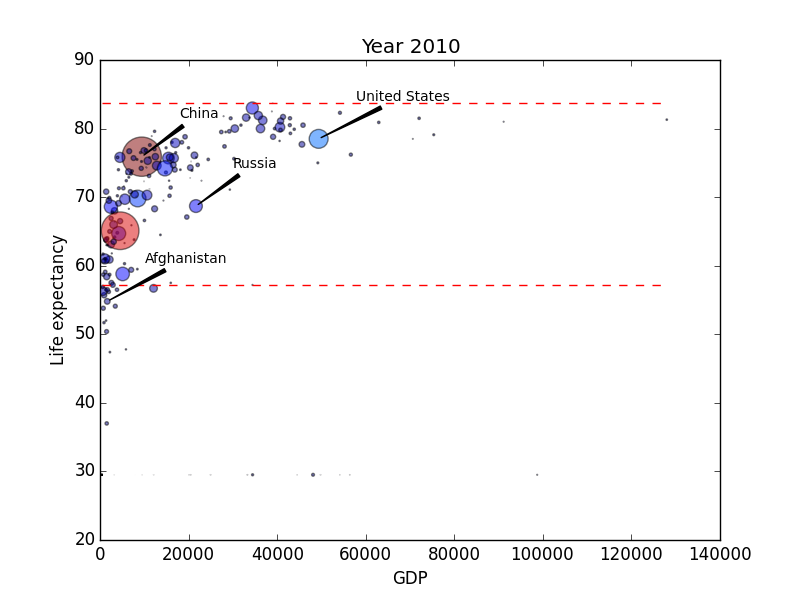
\includegraphics[width=\textwidth]{img/scatter_2010.png}
\end{center}
\end{ex}

\begin{infobox}{Supplementary Files}
The \texttt{country\_data.py} file is available on canvas.
\end{infobox}

\section{The CSV Module}
CSV files are used to store tabular data. They have comma separated values on
each line. Most spreadhseet programs support CSV output and input. Python comes
with the CSV module for reading and writing such files. It supports any
delimiter so you can also manage space-separated and tab-separated data. To
use the module, create a CSV reader using the filename of the data file. For
example, suppose we have the file \texttt{short.csv}. It has column labels
on the first row and columns are separated by commas.

\begin{verbatimcode}
Entity,x         ,y,  z
Fruit tree,1,2,3
Bats, 1, 3, 10
\end{verbatimcode}

We can use the \pythoninline{csv.DictReader} function to parse this data.
It takes an open file as the first argument and returns something that you
can use a for-loop to traverse. It essentially returns a list of dictionaries.
For example,

\begin{pyconcode}
>>> import csv
>>> with open('short.csv') as f:
...     l = [e for e in csv.DictReader(f)]
>>> print(l)
[{'Entity': 'Fruit tree', 'x': '1', 'y': '2', 'z': '3'},
 {'Entity': 'Bats', 'x': ' 1', 'y': ' 3', 'z': ' 10'}]
\end{pyconcode}

Read the documentation to learn about writing CSV files and the
\pythoninline{csv.Sniffer}, which can be used to deduce the format of
a CSV file.

\begin{center}
\url{https://docs.python.org/3/library/csv.html}
\end{center}

\section{Extra Credit Exercise}
\begin{extraex}[parsecsv.py]
The data in the \texttt{plotcountries.py} exercise is from
\url{http://www.gapminder.org/data/}. It was converted to CSV and
parsed using Python's CSV module. See the extra credit if you are
interested in this.  Parse these three CSV files using the CSV module.

\begin{itemize}
\item ``\texttt{indicator gapminder gdp\_per\_capita\_ppp.csv}''
\item ``\texttt{indicator gapminder population.csv}''
\item ``\texttt{indicator life\_expectancy\_at\_birth.csv}''
\end{itemize}

Your data should be the same as the \pythoninline{data} variable in
the \texttt{country\_data.py} file.
\end{extraex}

\begin{infobox}{Supplementary Files}
The following files are available on canvas:
``\texttt{indicator gapminder gdp\_per\_capita\_ppp.csv}'',
``\texttt{indicator gapminder population.csv}'',
and ``\texttt{indicator life\_expectancy\_at\_birth.csv}''.
\end{infobox}


\newpage
\section{Submitting}

You should submit your code as a tarball. It should contain all files
used in the exercises for this lab. The submitted file should be named
\begin{center}
  \texttt{cse107\_firstname\_lastname\_lab9.tar.gz}
\end{center}

\begin{center}
  \textbf{Upload your tarball to Canvas.}
\end{center}

\listofexercises
\listofextraexercises

\end{document}


